

\begin{frame}
    \frametitle{Performance Measures - Blocking time}
    \centering
    \begin{equation*}
        B = \frac{\sum_{(u,v) \in S_A^{(2)}} \pi_{(u,v)} \; 
        b(u,v)}{\sum_{(u,v) \in S_A^{(2)}} \pi_{(u,v)}}
    \end{equation*}

    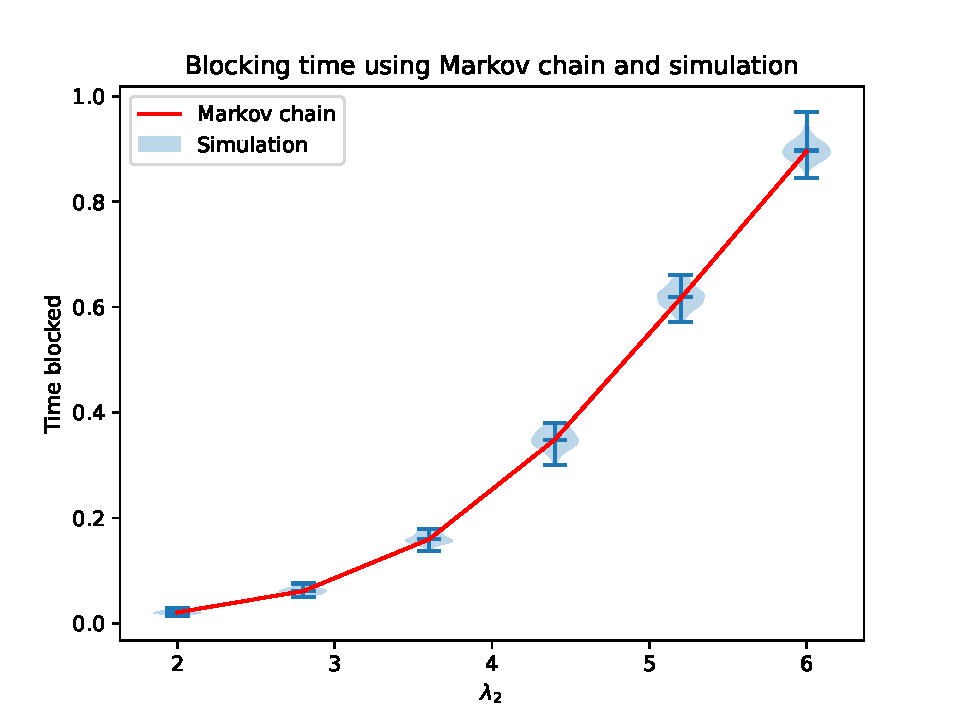
\includegraphics[scale=0.5]{Bin/performance_measures_comparison/blocking_comparison.pdf}

\end{frame}


\begin{frame}
    \frametitle{Performance Measures - Proportion within target}
    \centering
    
    \small
    \begin{equation*}
        P(W < t) = \frac{\lambda_1 P_{L'_1}}{\lambda_2 P_{L'_2}+\lambda_1 P_{L'_1}} 
        P(W^{(1)} < t) + \frac{\lambda_2 P_{L'_2}}{\lambda_2 P_{L'_2} + 
        \lambda_1 P_{L'_1}}P(W^{(2)} < t) 
    \end{equation*}


    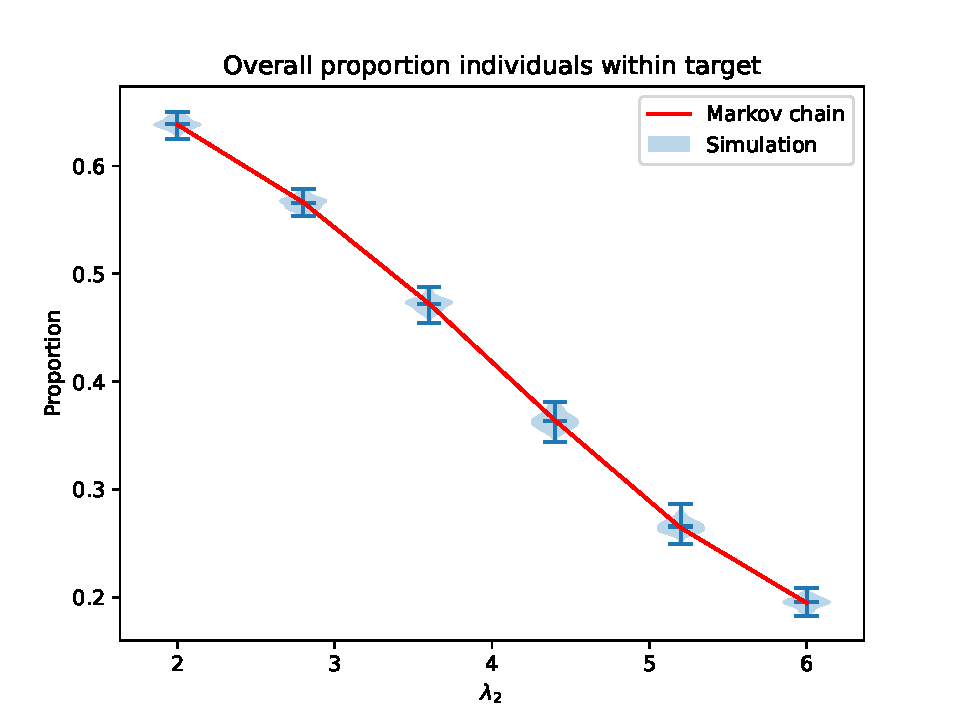
\includegraphics[scale=0.5]{Bin/performance_measures_comparison/proportion_overall_comparison.pdf}
    
\end{frame}


